%        File: ivarhs.tex
%     Created: Fri May 01 03:00 PM 2015 C
% Last Change: Fri May 01 03:00 PM 2015 C
%
\documentclass[a4paper, fleqn]{amsart}
\usepackage[]{palatino} 
\usepackage[]{mathpazo} 
\usepackage[]{microtype} 
\usepackage[]{amsmath} 
\usepackage[margin=1in]{geometry} 
\usepackage[]{mathtools} 
\usepackage[]{minted} 
\mathtoolsset{centercolon}

\newtheorem{prb}{Problem}
\theoremstyle{definition}
\newtheorem{sltn}{Solution}

\title{
  Mandatory Assignment 2 \\
  STK1100
}
\author{
  Ivar Stangeby
}
\begin{document}

\maketitle
\begin{prb}
  We let $X$ denote the yearly salary for a person chosen at random. We further
  assume that $X$ is Pareto distributed. The Pareto probability distribution
  has the density function:
  \begin{equation}
    \notag
    f_X(x) = \begin{cases}
      \theta\kappa^{\theta}x^{-\theta - 1} & \text{if } x > \kappa \\
      0 & \text{otherwise}.
    \end{cases}
  \end{equation}
  The quantity $\kappa$ is the minimum salary, where as $\theta > 2$ is a
  parameter dependent on the differences in salary.
\end{prb}

\begin{sltn}
\item\paragraph{a)}
  We want to find the cumulative probability distribution $F_X(x)$ of $X$.
  This is defined as
  \begin{equation}
    \notag
    F_X(x) = P(X \leq x) = \int_{-\infty}^{x}f_X(y) \, dy, 
  \end{equation}
  however since $f_X(y)$ contributes nothing to the integral when $y$ is in the
  range $(-\infty, \kappa)$.  We can therefore evaluate the integral
  \begin{align*}
    \notag
    F_X(x) &= \int_{\kappa}^{x}f_X(y) \, dy.\\
    &= \theta\kappa^{\theta}\int_{\kappa}^{x}y^{-\theta-1} \, dy  \\
    &= \theta\kappa^{\theta} \Big\lvert -x^{-\theta} \Big\rvert_{\kappa}^{x}\\
    &= \kappa^{\theta}\kappa^{-\theta} - \kappa^{\theta}x^{-\theta} \\
    &= 1 - \kappa^{\theta}x^{-\theta}, 
  \end{align*}
  as required.

  The \textit{median yearly salary} is the real value $m$ that satisfies
  \begin{equation}
    \notag
    F_{X}(m) = \frac{1}{2}.
  \end{equation}
  Solving this equation for $m$ gives
  \begin{equation}
    \notag
    m = \sqrt[\theta]{2}\kappa.
  \end{equation}

\paragraph{b)}
We want to find the expected value of $X$. This is given by
\begin{equation}
  \notag
  \mathbb{E}\left[ X \right] = \mu_{X} = \int_{\kappa}^{\infty} xf_X(x)\, dx= \lim\limits_{b\rightarrow\infty}\int_{\kappa}^{b}xf_X(x)\, dx
\end{equation}
Evaluating the last integral gives us
\begin{equation}
  \notag
  \lim_{b\rightarrow\infty}\theta\kappa^{\theta}\Big\lvert \frac{x^{-\theta + 1}}{-\theta + 1}\Big\rvert_{\kappa}^{b},
\end{equation}
which in turn equals
\begin{equation}
  \notag
  \mathbb{E}\left[ X \right]= \frac{\theta\kappa}{\theta-1}
\end{equation}

\paragraph{c)}
Given $\kappa = 200000$ and $\theta = 2.5$ we evaluate the median yearly salary and the expected yearly salary:
\begin{equation}
  \notag
  m = \sqrt[\theta]{2}\kappa \approx 263901, 
\end{equation}
\begin{equation}
  \notag
  \mathbb{E}\left[ X \right] = 333333,333\dots.
\end{equation}
The median yearly salaray better captures the skewness in the salary
distribution across a population, where as the expected value is biased towards
the low amount of people earning most of the money.

\paragraph{d)}
We want to find the variance and standard devation of $X$. These are given by
\begin{equation}
  \notag
  \mathbb{V}\left[ X \right] = \mathbb{E}\left[ (X - \mu)^2 \right] = \mathbb{E}\left[ X^{2} \right] - \mu_X^{2}, 
\end{equation}
\begin{equation}
  \notag
  \sigma = \sqrt{\mathbb{V}\left[ X \right]}.
\end{equation}
The variance is easily derived as
\begin{equation}
  \notag
  \mathbb{V}\left[ X \right] = \lim\limits_{b\rightarrow\infty}\int_{\kappa}^{b}x^{-\theta+1}\, dx - \mu_X^{2}.
\end{equation}
Solving this integral yields:
\begin{equation}
  \notag
  \mathbb{V}\left[ X \right] = \frac{\kappa^{2}\theta}{\theta - 2} - \mu_X^{2} = \frac{\theta\kappa^2}{(\theta-2)(\theta-1)^2}
\end{equation}
\begin{equation}
  \notag
  \sigma = \frac{\sqrt{\theta}\kappa}{\sqrt{(\theta-2)}(\theta -1)}
\end{equation}

\paragraph{e)} If we let $Y  = \theta\ln(X/\kappa)$ and we solve for $X$ we get
\begin{equation}
  \notag
  X = \kappa e^{y/\theta}.
\end{equation}
Substituting this into the probability density function for $X$, we get the following density function:
\begin{equation}
  \notag
  f_{Y}(y) = \theta\kappa^{\theta}\left( \kappa e^{y/\theta} \right)^{-\theta - 1}, 
\end{equation}
which simplifies to
\begin{equation}
  \notag
  f_{Y}(y) = \frac{\theta}{\kappa} e^{-\left(1 + \frac{1}{\theta}\right)y}, y > 0.
\end{equation}
which we recognice as the \textit{exponential} distribution.
\end{sltn}

\begin{prb}
  We let $X_1, X_2, \dots, X_n$ be independent and identically distributed
  random stochastic variables, i.e., their probability distributions are the
  same. We also let $\mu = \mathbb{E}(X_i)$, and $\sigma^2 = \mathbb{V}(X_i)$.
  We introduce the arithmetic mean
  \begin{equation}
    \notag
    \overline{X_n} = \frac{1}{n}\sum_{i=1}^{n}X_i,
  \end{equation}
  and the standarized mean
  \begin{equation}
    \notag
    Z_n = \frac{\overline{X_n}-\mu}{\sigma/\sqrt{n}}.
  \end{equation}
\end{prb}

\begin{sltn}
\item\paragraph{a)} We want to show that $\mathbb{E}(Z_n) = 0$ and $\mathbb{V}(Z_n) = 1$. We know that
  $\mathbb{E}(\overline{X_n}) = \mu$ and that $\mathbb{V}(\overline{X_n}) = \sigma^2/n$.
  Starting with the expected value, we substitute the expression for $Z_n$ and find:
  \begin{align*}
    \notag
    \mathbb{E}(Z_n) = \frac{1}{\sigma/\sqrt{n}}\mathbb{E}(\overline{X_n}) - \frac{1}{\sigma/\sqrt{n}}\mu = 0.
  \end{align*}
  We use the similar approach for the variance $\mathbb{V}(Z_n)$.
  \begin{align*}
    \mathbb{V}(Z_n) = \frac{1}{\sigma^{2}/n}\mathbb{V}(\overline{X}) = 1
  \end{align*}

\paragraph{b)}
Starting with the uniform distribution, we have:
\begin{align*}
  &\mu = \mathbb{E}(X_i) = \int_{0}^{1}x \, dx = \frac{1}{2}\\
  &\sigma^{2} = \int_{0}^{1}x^{2}\, dx - \frac{1}{4} = \frac{1}{12}\\
  &\sigma = \frac{1}{2\sqrt{3}}
\end{align*}
The exponential distribution yields (using integration by parts):
\begin{align*}
  &\mu = \int_{0}^{\infty}xe^{-x} \, dx = 1 \\
  &\sigma^2 = \int_{0}^{\infty}x^2e^{-x} \, dx = 2 - \mu^2 = 1\\
  &\sigma = 1
\end{align*} 
The bernoulli distribution with paramter $p$ has
\begin{align*}
  &\mu = p = \frac{1}{2}\\
  &\sigma^2 = p(1-p) = \frac{1}{4}\\
  &\sigma = \frac{1}{2}
\end{align*}


\paragraph{c)}

According to the \textit{Central Limit Theorem} the standarized versions of
$\overline{X_n}$ will have the standard normal distribution.
\\
\paragraph{d)}
\begin{figure}[p]
  \centering
  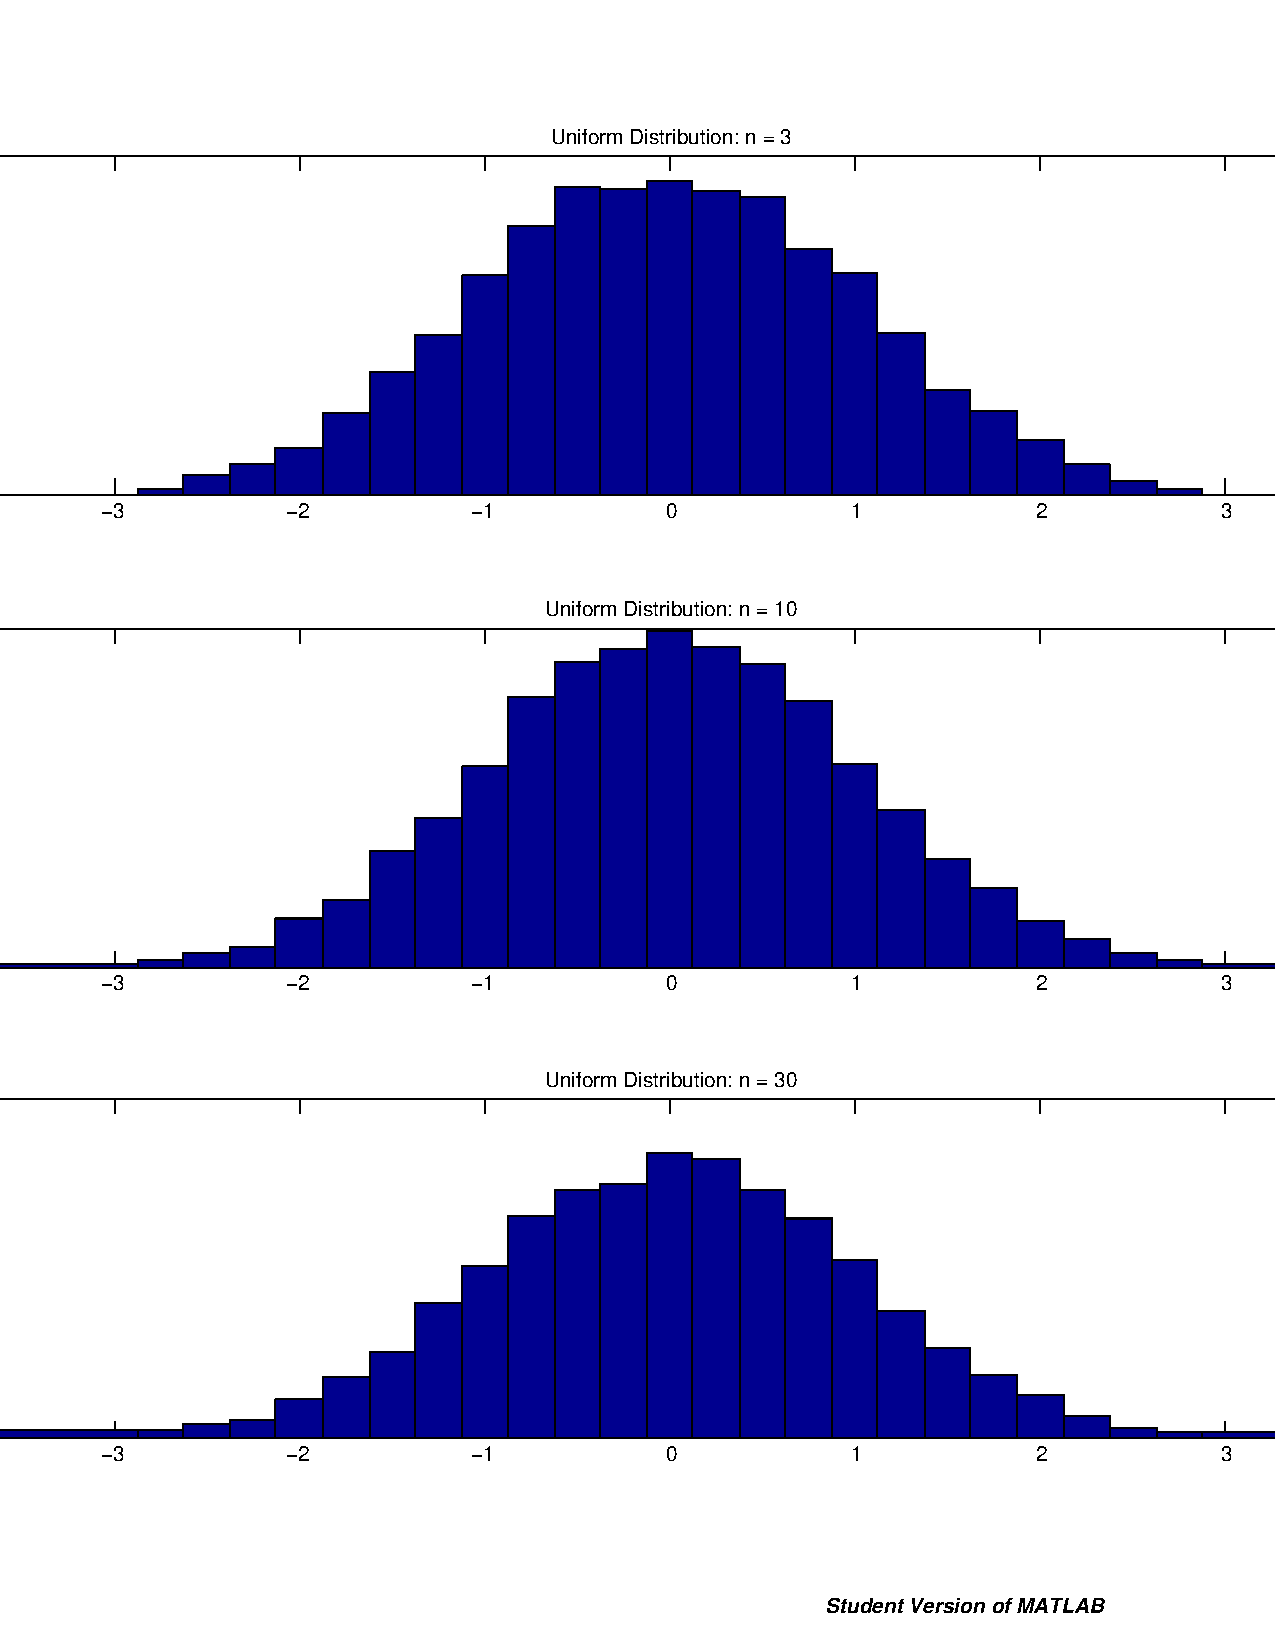
\includegraphics[scale=0.4]{uniform_mean}
  \caption{Standarized mean - Uniform Distribution}
  \label{fig:uniform_mean}
\end{figure}

Examining the first histogram in Figure \ref{fig:uniform_mean} we see that we
have something that looks like a normal distribution, however $n = 3$ is not
sufficient to get a good approximation. The higher the $n$ the more
concentrated the distribution is around $\mu$ according to the Central Limit Theorem
\\
\paragraph{e), f)}

The probabilities of standard normal distributed variable falling in 
any of these intervals are given in Figure \ref{fig:relative_frequencies}
\begin{figure}[p]
  \centering
  \label{fig:relative_frequencies}
  \begin{tabular}{c|c|c}
  Interval & Probability & Relative Frequency \\
  \hline
  $\left( -\infty, -2.5 \right]$ & 0.0062 & 0.0027\\
  $\left( -2.5, -2.0 \right]$ & 0.0166 & 0.0177\\
  $\left( -2.0, -1.5 \right]$ & 0.0440 & 0.484\\
  $\left( -1.5, -1.0 \right]$ & 0.0919 & 0.0930\\
  $\left( -1.0, -0.5 \right]$ & 0.1498 & 0.1570\\
  $\left( -0.5, 0 \right]$ & 0.1915 & 0.1897\\
  $\left[ 0, 0.5 \right)$ & 0.1915 & 0.1835\\
  $\left[ 0.5, 1.0 \right)$ & 0.1498 &0.1454\\
  $\left[ 1.0, 1.5 \right)$ & 0.0919 & 0.0920\\
  $\left[ 1.5, 2.0 \right)$ & 0.0440 & 0.0517\\
  $\left[ 2.0, 2.5 \right)$ & 0.0166 &0.0167\\
  $\left[ 2.5, \infty \right)$ & 0.0062 & 0.0022\\
\end{tabular}
\caption{Probabilities and relative frequencies}
\end{figure}
\paragraph{g)}
We see from Figure \ref{fig:uniform_mean} for $n = 10$ and $30$ that the
distribution looks more and more like the standarized normal distribution. This
is in accordance with the Central Limit Theorem. The relative frequencies
converges to the probabilities outlined in Appendix A.3.

\paragraph{h)}

\begin{figure}[p]
  \centering
  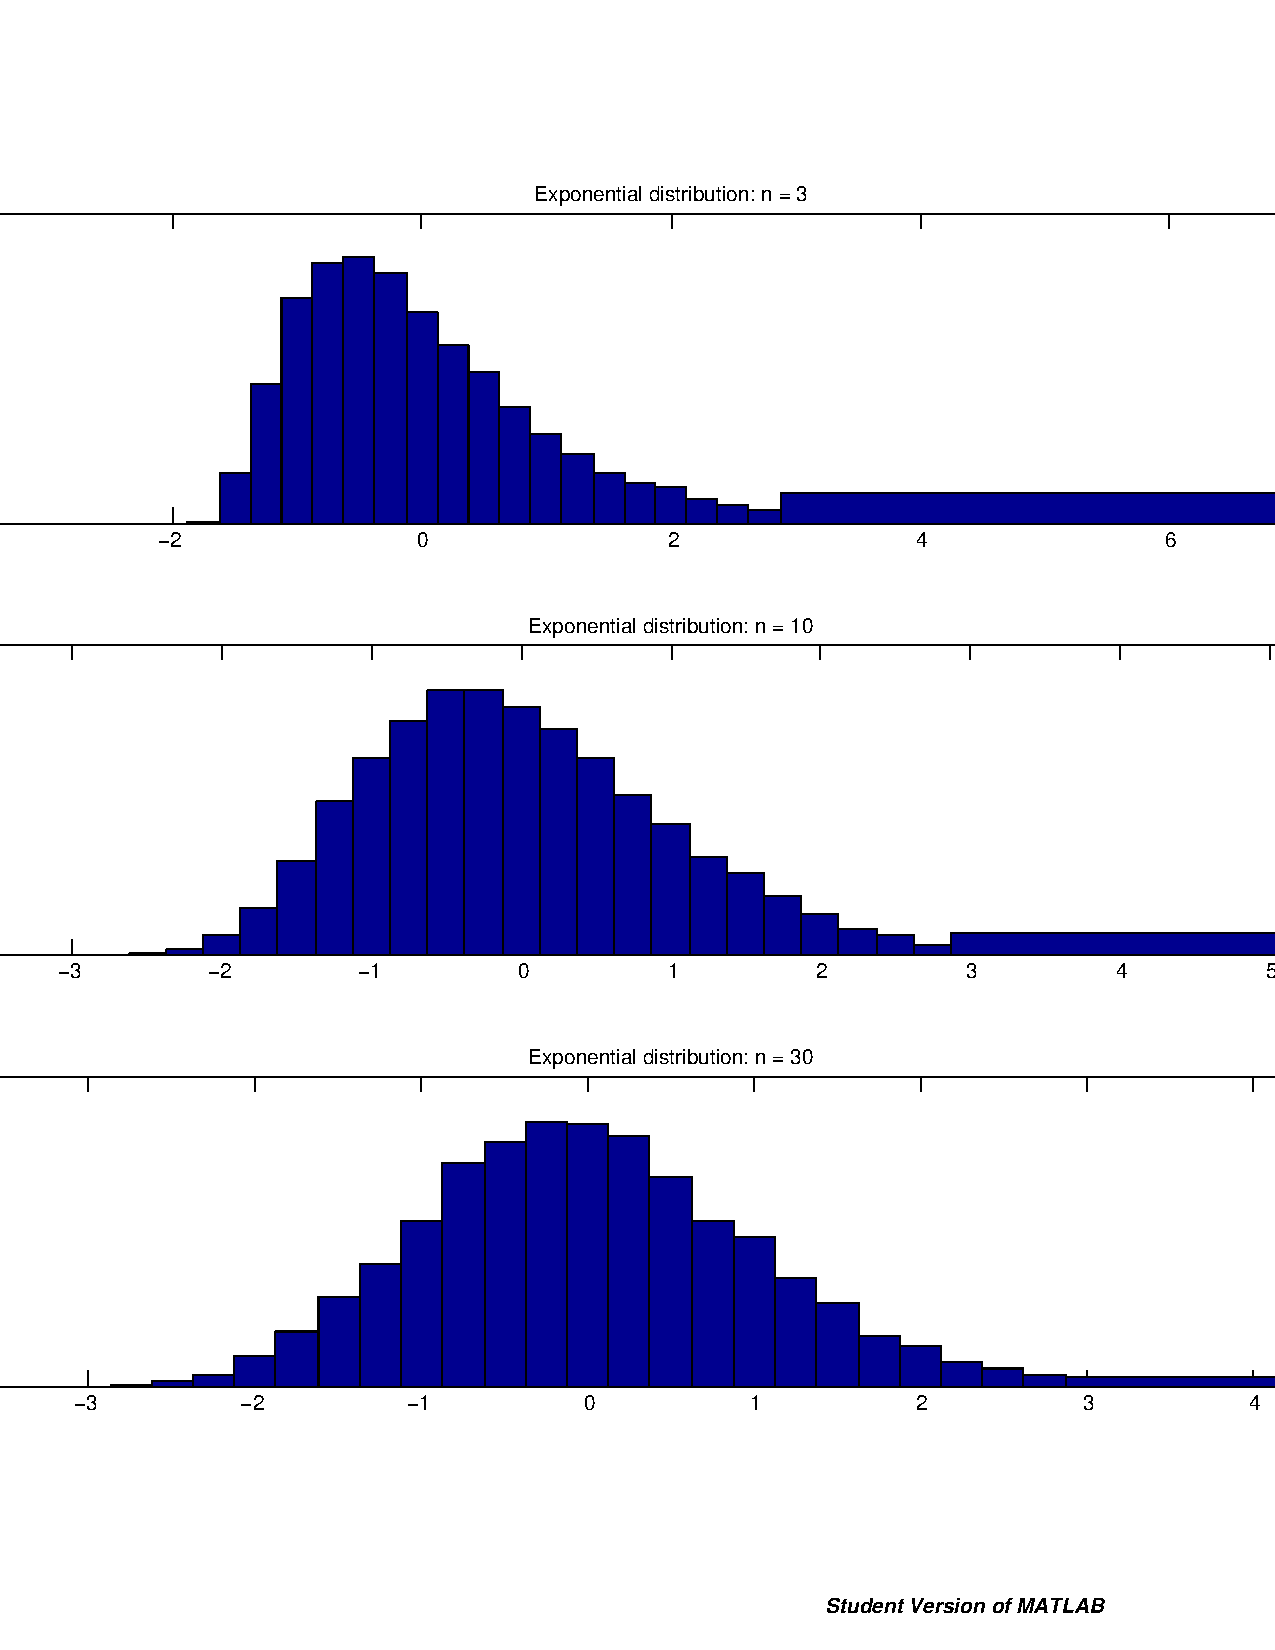
\includegraphics[scale=0.4]{exponential_mean}
  \caption{Standarized Mean - Exponential Distribution}
  \label{fig:exponential_mean}
\end{figure}

Nothing new to see here, again this is in accordance with the Central Limit Theorem.
The distribution converges to the standard normal distribution for increased values of $n$.
It is very skewed at $n = 3$. The relative frequences are also converging to the probabilities
in Figure \ref{fig:relative_frequencies}.

\paragraph{i)}

\begin{figure}[p]
  \centering
  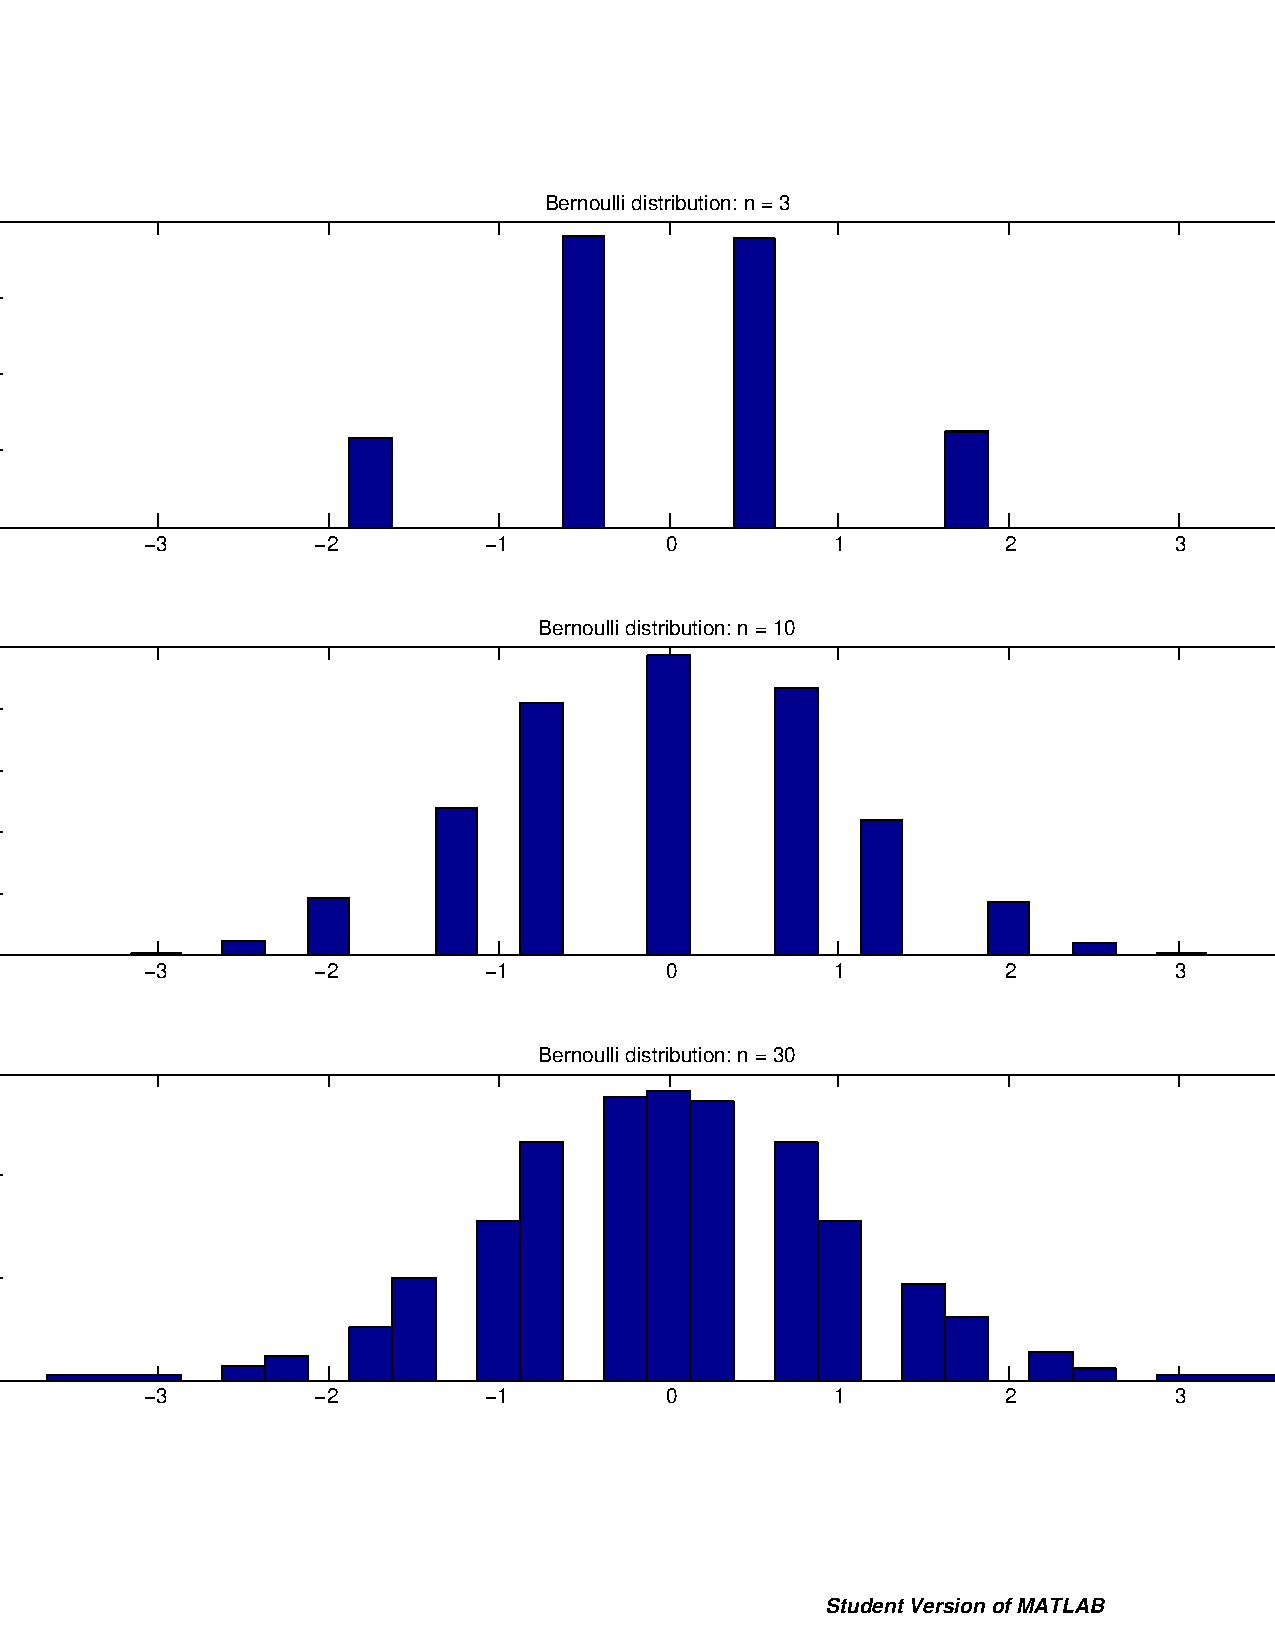
\includegraphics[scale=0.4]{bernoulli_mean}
  \caption{Standarized Mean - Bernoulli Distribution}
  \label{fig:bernoulli_mean}
\end{figure}

Again, according to the central limit theorem - this converges to the standard
normal distribution for increasing values of $n$. 

\paragraph{j}

It is definitely the uniform distribution that gives us the standarized mean
that is closest the the standard normal distribution for the values $n = 3, 10,
30$. However if we let $n \rightarrow \infty$, we should see a similiar
distribution for all of the standarized means.
\end{sltn}

\begin{prb}
  Letting $X_1, \dots, X_9$ be independent random variables with identical
  distribution $F$. The \textit{empirical mean}, 
  \begin{equation}
    \notag
    \overline{x} = 56.22, 
  \end{equation}
  and the median, 
  \begin{equation}
    \notag m(x_1, \dots, x_9) = 46, 
  \end{equation}
  are both two natural estimations. We are going to examine these estimators by looking
  at their properties.
\end{prb}
\begin{sltn}
\item\paragraph{a)} 
We want to find the standard error $SE$ and the expectation scewness for the
two estimators. We do this using \textit{non-parametric bootstrapping}. The
empirical standard deviation $\hat{\sigma} = 42.48$.  The simulations yields
a standard error of $\approx 13,2$ for the median estimator, and $\approx
13,4$ for the mean estimator.

The bias of the mean is very low at $\approx -0.0150$, probably due to the fact
that the variables are independent, where as the bias for the median is
slightly larger at $\approx -0.1148$.

\paragraph{b)}
\begin{figure}[p]
  \centering
  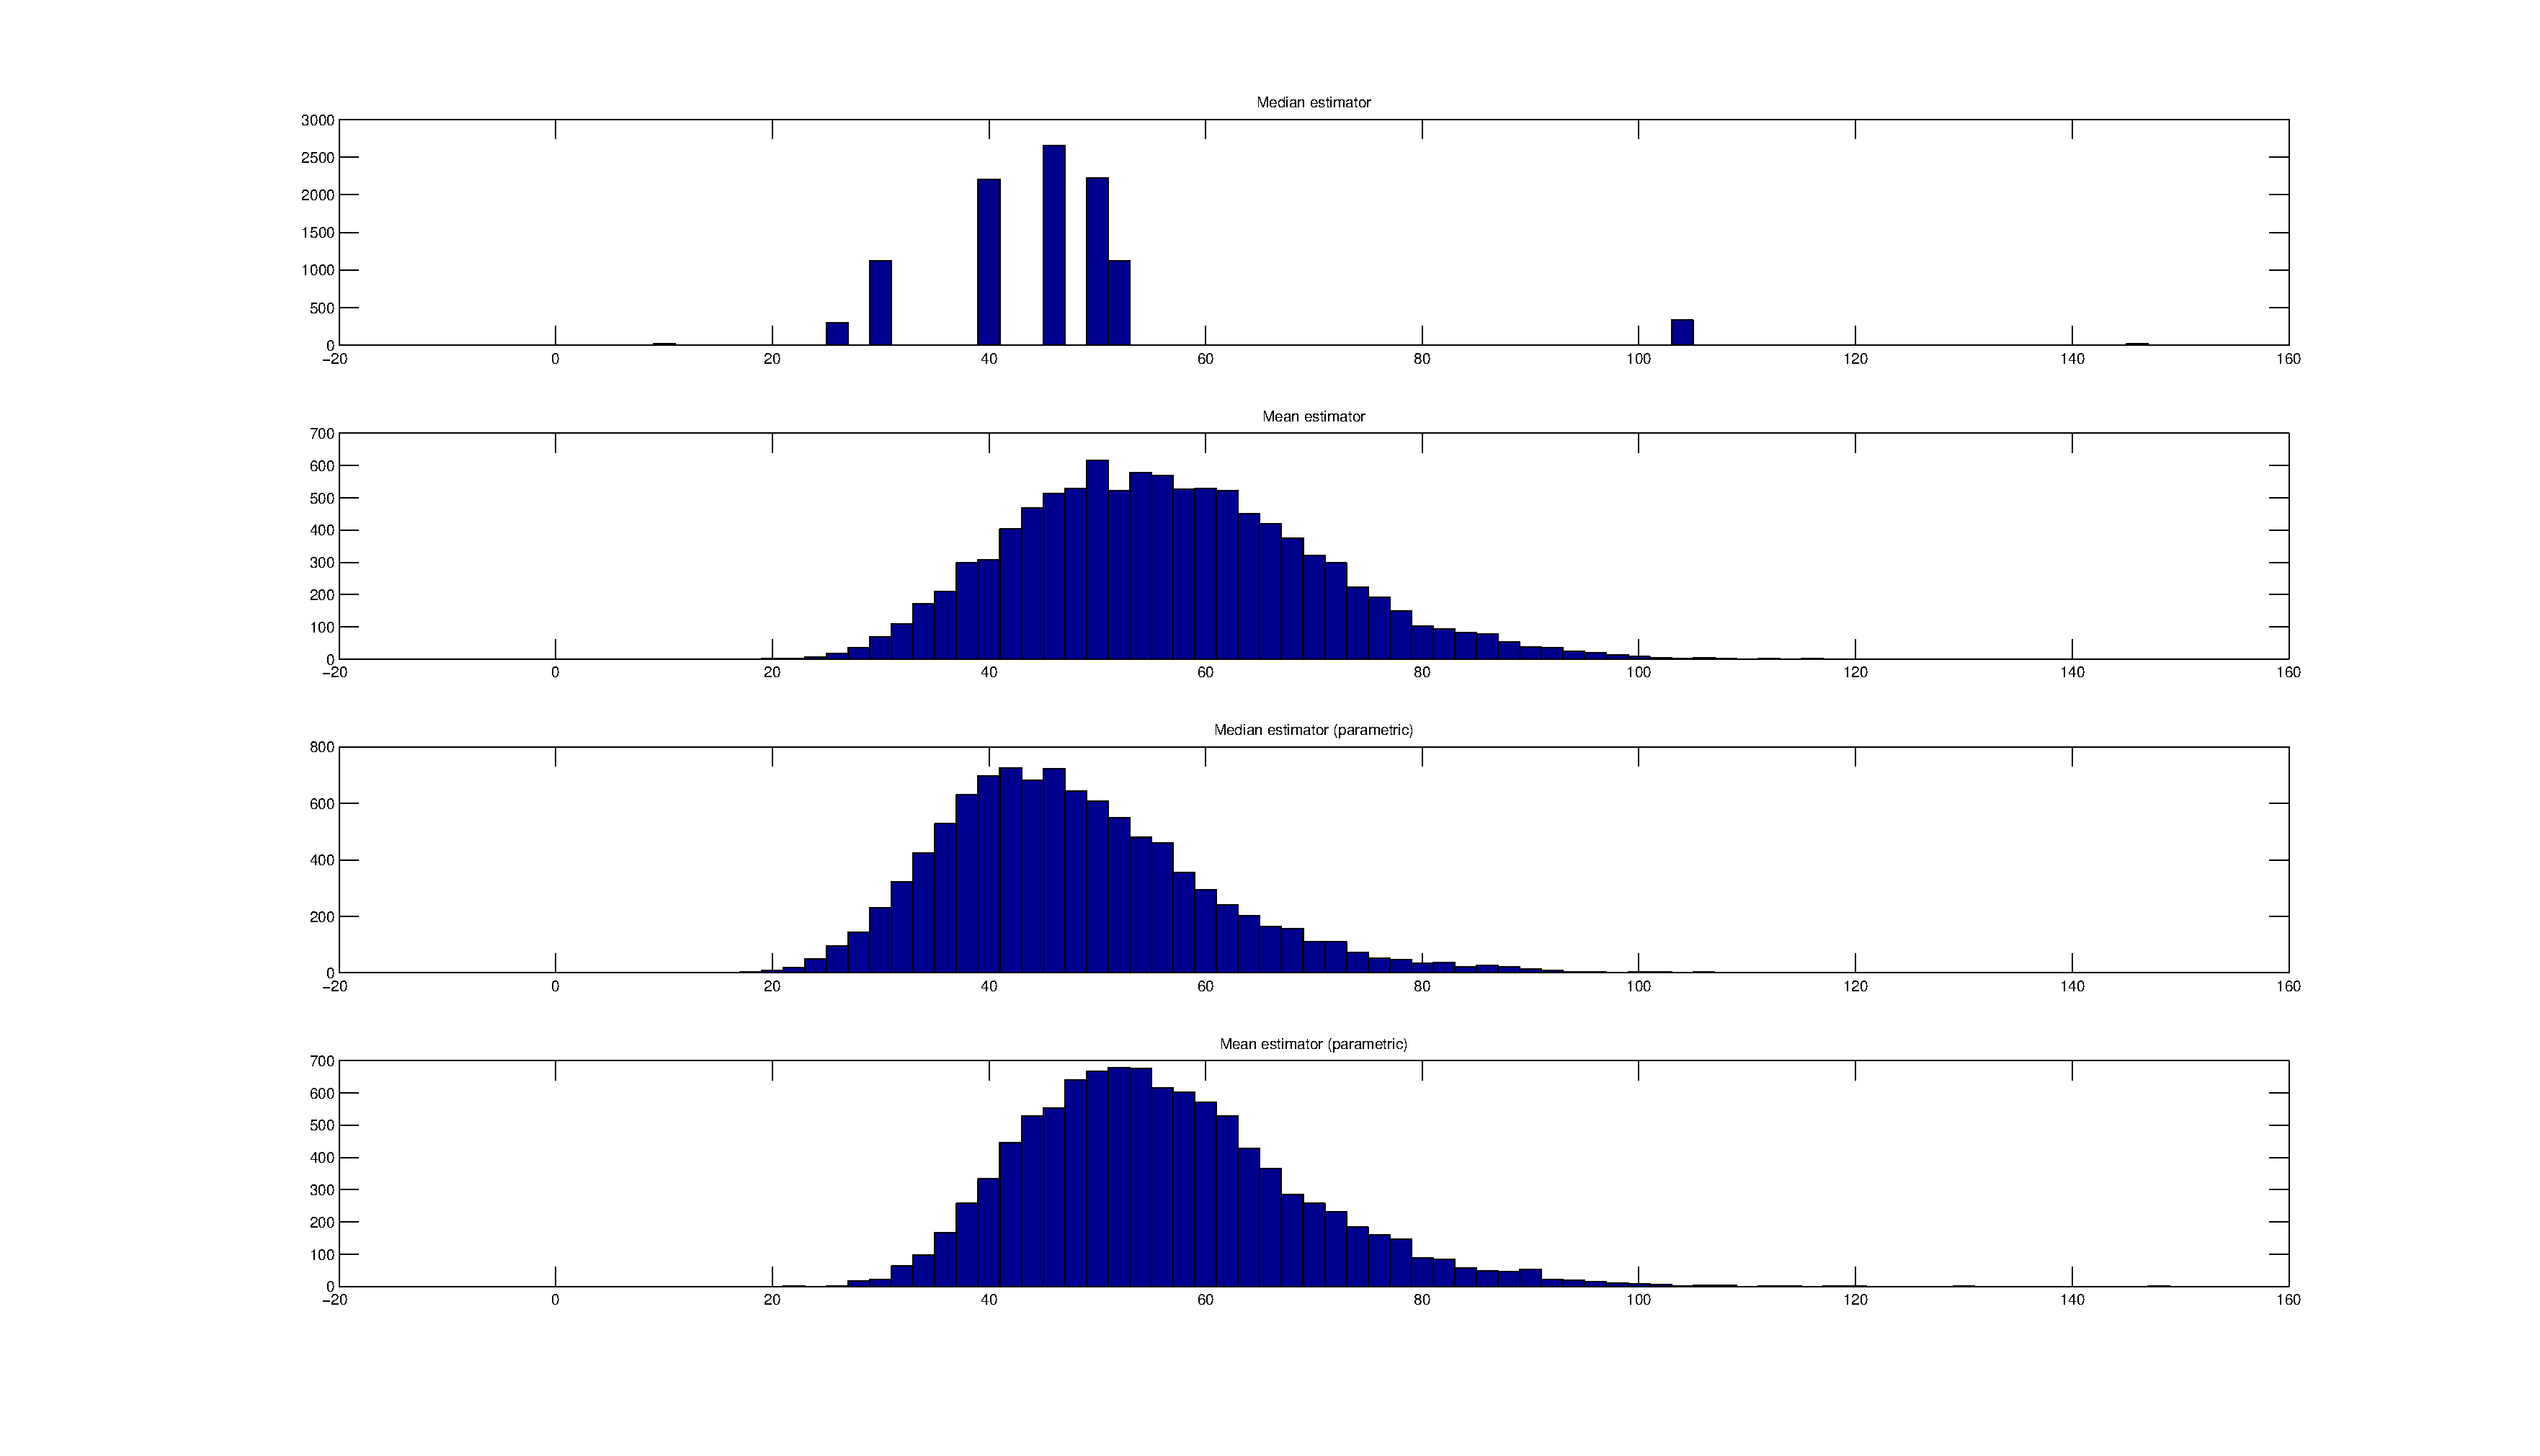
\includegraphics[scale=0.3]{estimators_histogram}
  \caption{Histograms of the two estimators}
  \label{fig:estimator_histogram}
\end{figure}
The estimator for the median of the distribution, as shown in Figure
\ref{fig:estimator_histogram} looks the way that it does, because the median is
defined as the observation that splits the whole samplie into two halfs, the
greater and the lesser. The histogram of the estimator for the mean does look
log-normally distributed.

\paragraph{c)} If we now assume that the random variables are log-normally distributed, we know
that the median is given by
\begin{equation}
  \notag
  e^\mu, 
\end{equation}
and the mean is given by
\begin{equation}
  \notag
  e^{\mu + \sigma^2 / 2}.
\end{equation} where
$\mu$ is the location of the distribution, and $\sigma$ is the scale. We want
to perform parametric bootstrapping on the random variables $X_1, \dots, X_9$
in order for us to see whether our prediction is reasonable.

A reasonable estimator for the median is going to be
\begin{equation}
  \notag
  e^{\hat{\mu}}
\end{equation} and
for the mean
\begin{equation}
  \notag
e^{\hat{\mu} + \hat{\sigma}^2 / 2}
\end{equation}
with $\hat{\mu} = mean(x)$ and $\hat{\sigma}^2 = SE(mediansim)^2$
\end{sltn}
The result of the parametric bootstrap is shown in Figure \ref{fig:estimator_histogram}.
\inputminted{matlab}{~/Documents/MATLAB/STK_Oblig2.m}

\end{document}


